\section{Discussion}
\label{Discussion}
\textbf{FIXME: La conclusione la incorporo come subsection della discussion o la tengo separata? }\\
In this section we discuss the results of the transformation, its feasibility and the possible future developments. We also present a use case to show how the generator works on a simple transformation.
\subsection{Emulate a BPEL Orchestration in Java}
\label{sec:OrchestrEmulation}
Our purpose was to show the feasibility of an automatic transformation from a BPEL orchestrated process to a Java application. With the use of a model-to-text methodology we met the intent and we provide a simple implementation of a proof of concept showing.
On the functionality of the transformation, obvious constraints have been set. First, not to overcome the complexity due to the wide structure of the BPEL language, we use a subset of the language. Second, we limit the focus to only one workflow pattern. 
These constraints have been set not to overcome the project time-frame.


\subsection{Use Case}
\label{sec:UseCase}
Here we provide a simple use case to show how the generator works. Figure \ref{fig:GeneratorUseCase} represents a scenario where a user inputs a BPEL model and receives in output the Java application mimicing the BPEL orchestration.
The use case can be described as follows:
\begin{itemize}
 \item The runs the generator, which includes:
  \subitem Insert a BPEL input (complying with out pattern) 
  \subitem Manually set the Variables' names and types
  \subitem Run the wsimport() routine on the WSDL files.
\end{itemize}
Once the generation has completed, the user of the Java application can finally:
\begin{itemize} 
 \item Run the Java application (creating an instance of it and run the \textit{runWorkflow()} method), which includes:
  \subitem Manually set the web service invocation.
\end{itemize}

\begin{figure}
  \begin{center}
    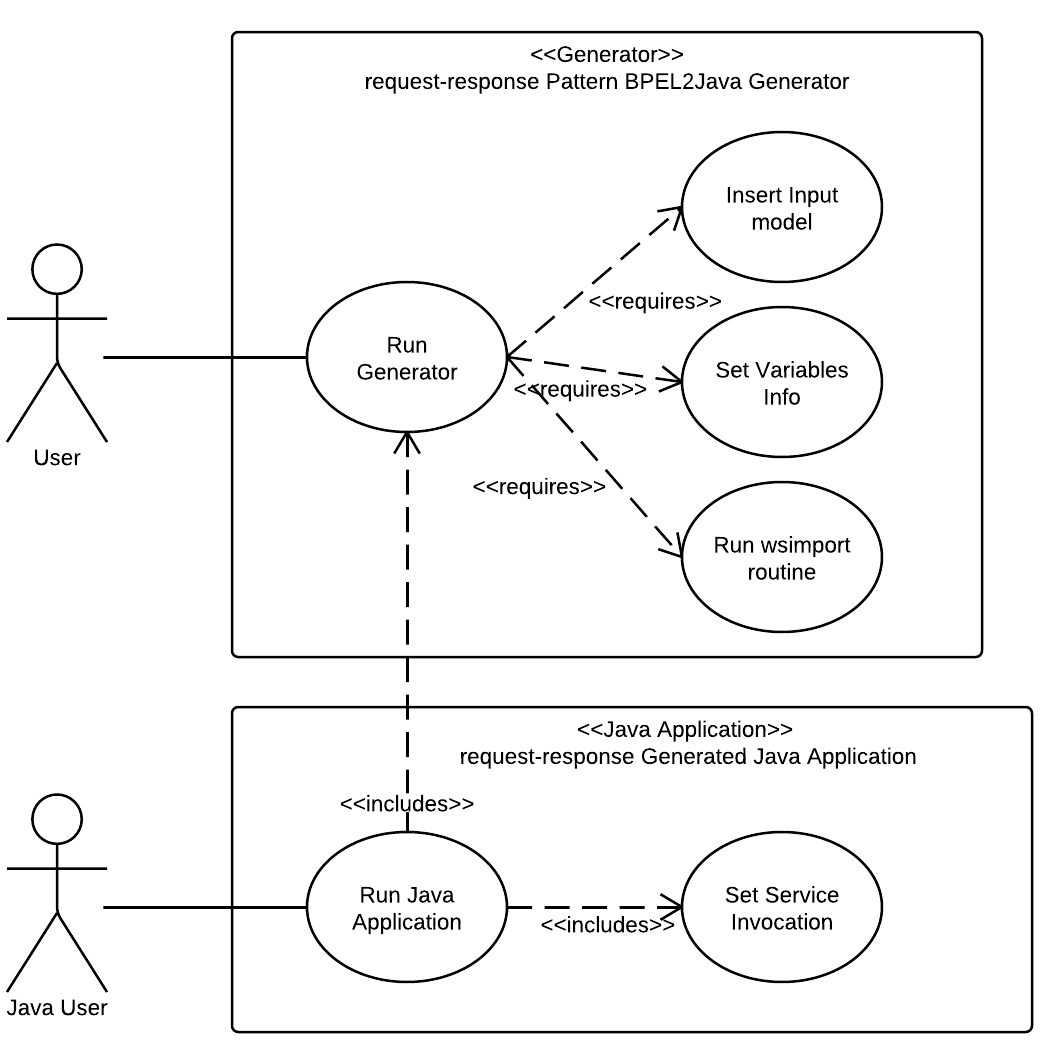
\includegraphics[scale=1.5]{pictures/GeneratorUseCase.png}
    \caption{Use Case of the BPEL to Java generator}
    \label{fig:GeneratorUseCase}
  \end{center}
\end{figure}

\subsection{Future Development}
\label{sec:FutureDevelopment}
This Section briefly shows the possible improvements and future development that might be carried out on the BPEL to Java transformation.

\subsubsection{Retrieve information from WSDL files}
\label{sec:FutRetrieveWSDLInfo}
As previously described in Section \ref{sec:issues}, some technical issues mainly due to the impossibility of providing more than one input models to the Acceleo generator, made us redefine the design and contemplate a developer's intervention 
for anything that concern the WSDL files.
We think that if the information from the WSDL file would be available, the developer's intervention would be much less needed, and error-prone manual operations (like rewriting or copy-pasting the, often long, WSDL elements fields) would be avoided. 
We forecast a possible future development undertaking two ways:
\begin{enumerate}
 \item \label{itm:num1}modify the Acceleo API and implementation
 \item \label{itm:num2}recur to Java properties file 
\end{enumerate}

\paragraph{Modify the Acceleo tool}
Concerning the point number \ref{itm:num1}, modifications to the Acceleo API and its implementation could be made, though at a high cost in terms of time and knowledge to acquire concerning the Acceleo's internal mechanisms. As the Acceleo developers responded us on the official forum: the modifications would not be a trivial task.
Moreover, we don't know if the developers would take into considerations the option of rising the number of possible input files. This because the majority of Acceleo users tend to run the same transformation over several input models of the same kind (e.g. batch transformation of UML diagrams in Java) while a case like ours, where coordination among input models is required (BPEL and WSDL files), it is not common.

\paragraph{Java properties file}
A simpler idea to overcome the problem of accessing the WSDL file would be to create another Acceleo transformation (parameterized by the WSDL meta-model) taking as input a WSDL file. From here we could get the needed information and write them out in a Java Properties file. A Java properties file, as shown in the Listing \ref{lis:JavaPropertyFile}, is a very simple text file containing some variables and their values. It is usually provided to a Java application when some parameters have to be set manually, like, for example, the absolute path to some local resources.

\begin{center}
  \begin{minipage}{1\textwidth}
    \begin{java-code}{Example of a Java properties file}{lis:JavaPropertyFile}
#Mon Aug 31 12:50:43 GMT 2012
ElementType=Person
ElementName=Employee
database=localhost
user=process
    \end{java-code}
  \end{minipage}
\end{center}

Once we would have written the information from the WSDL file in the Java properties file, we could use the Acceleo facility that permits to input a Java properties file with the command:\\
\begin{verbatim}[getProperty('myroperty')/]\end{verbatim} 
The usage of properties file in Acceleo is described in the documentation \cite{acceleoDoc}. If the WSDL files are more than one (e.g. presence of more than one PartnerLink), the transformations could be run more times attaching the new information at the end of the properties file.
This improvement would basically overcome both the issues presented in Section \ref{sec:issues}.

\subsubsection{Include more BPEL patterns}
\label{sec:FutMorePatterns}
Our transformation focuses on only one kind of BPEL workflow patten, namely, a sequence of "receive - assign - invoke - assign - reply". More patterns could be added, especially working on simple variants of some basic ones. A good source of information on workflow patterns, is the Article from W.M.P. Vand Der Aalst et. al. \cite{AalstHKB03}; here the workflow patterns are abstracted from the modeling tools, so that they can be generalized, spotting commonalities and differences among them.
Eventually, transformations addressing different workflow patterns could be, either contained in their own generator, or be a specialization of another pattern. For example, a pattern where a final reply must be sent to two PartnerLinks (two BPEL \textit{reply}s), could be a special case of the one where there is only one reply to one PartnerLink.    

\subsubsection{Improve architectural design for additional Patterns}
\label{sec:FutImproveArchitectDesign}
Once the set of BPEL patterns would be enlarged, it will be necessary to improve the code reuse and add some abstraction layers to the architecture of both the Acceleo transformation and the Java application. Some of the ideas could be to use Acceleo modules hierarchies (see Table \ref{tab:terminology} on the Acceleo terminology) to specialize some of the operations. For example, one could be in need to create different PartnerLink STUBs depending on the type or role of the PartnerLink. The same happens with the Java application, where PartnerLinks STUBS could be implementing a generic PartnerLink interface class. 
